\documentclass[../../../main.tex]{subfiles}
\begin{document}

%\subsection{Capabilities and limitations of the stochastic structure generation algorithm}

Much effort was made to improve the algorithm so that it can handle and adapt to as many geometries as possible, but not all geometries are accepted. 
Below are described the geometries that were successfully accepted, along with the conditions that a geometry must meet to be processed by the algorithm. 
It should be noted that the limitations described are those presented by the algorithm at the time of writing this manuscript.

\subsubsection{Flat upper and lower bases}
During the first steps of the algorithm, the lower section of the volume is extracted, from which the structure begins to be generated. 
Therefore, the geometry to be processed must have a flat base.
Otherwise, the algorithm cannot begin. 
Something similar happens with the upper part of the geometry: the termination criterion moves the vertices generated in the last layer to the highest \textit{z}-coordinate of the geometry. 
Therefore, if the upper base is not flat, there could be edges that cross the upper part of the geometry and remain outside it. 

\subsubsection{Pronounced curvatures}
The height of the tetrahedra depends mainly on the size of the base and the minimum angle set. 
The larger the base, the larger the tetrahedron. 
This means that the tetrahedra have a minimum size and cannot adapt to geometries with very pronounced curvature with any pore size. 
In addition, the geometry must have a straight vertical axis, although it can be inclined. 
Once a new generation of tetrahedra has been generated, to orient the growth vectors, the algorithm studies the variation of the surface at greater heights, but it does so by obtaining horizontal sections of the surface. 
The vectors are then oriented according to that result. 
For example, a C-shaped geometry would not be acceptable because there are areas where the inclination of the vectors must vary by nearly 90$^\circ$, and this would not be correctly captured by making horizontal sections.
The sections should be made in a guided manner along the spine of the volume to capture changes in the orientation of the geometry. 
 
\subsubsection{Significant changes in local topology}
Similar to the previous limitation, very abrupt changes in geometry would not be captured correctly. 
Even if they can be accepted, the results would not be correct. 
For example, in a T-shaped geometry, the increase in the section when changing from the vertical to the horizontal region is so huge that the tetrahedra generated in the transition region increase greatly in area and, therefore, in height, and would probably be generated entirely outside the volume.

\subsubsection{Large pore sizes}
As mentioned above, the pore size is established by generating several triangles in the first section such that their average area is equal to the pore size. 
The fewer polygons there are, the larger the pore area will be. 
However, the number of triangles can never be zero, since to create these triangles, points extracted from the surface of the volume are used, along with others generated in order to achieve the established pore size.
Therefore, depending on the number of points present on the perimeter of the extracted section, more or fewer triangles can be generated. 
However, it will never be possible to generate fewer triangles than those that result from triangulating the points on the perimeter themselves. 
Therefore, the pore size will be limited by the number of points present on that perimeter.
And the limit will be the average area of the triangles resulting from triangulating the points in the section. 
It is difficult to establish a relationship between the maximum size and the number of points extracted, as it depends on several factors such as the edge length of the imputed mesh, the geometry of the section and the size. 
Therefore, each case will be different. 
On the other hand, there is no lower limit, as more points can always be added to obtain the pore size.

Despite the limitations described, the algorithm is capable of supporting a multitude of geometries. 
From geometries with holes to variable section geometries, even inclined ones. 
A hole detection module for screws was included, allowing them to be supported in the geometries. 
This demonstrates not only that it is capable of detecting small holes and adapting to them, but also that holes of various sizes can exist in the geometry. 
Even the coexistence of through holes with blind holes is possible. 
In the current state of the algorithm, the supported geometries are those that could be used in real-world problems. 
Geometries that are not supported are unusual ones that are not so common in industrial applications.
Below are some examples of structures generated in different geometries.

\subsection{Printability of the generated structures}

So far, reference has been made to virtual structures, as it has not yet been verified whether the designed structures actually achieve their purpose: to be 3D printable without support. 
Below are several images of 3D-printed structures.
Three different technologies were used to print the structures: stereolithography  (SLA), fused filament fabrication (FFF) and laser powder bed fusion (LPBF).
For SLA printing, an ELEGOO Saturn 3D printer and a standard resin (grey, UV 405 \textit{nm}, ELEGOO) were used. 
The layer thickness was set to 0.05 \textit{mm}, and a normal layer exposure time of 2.5 seconds was used.
For FFF, a Creality Ender 3 V1, PLA and 200$^\circ C$ nozzle temperature, 0.1 \textit{mm} layer height and 20 \textit{mm/s} print speed were used. 
Metal printing was delegated to the National Centre for Metallurgical Research (Madrid, Spain). 
The material used was Ti6Al4V, and a TruPrint 1000 printer was used.
Only three samples were printed due to the high cost of printing of this technology.
The pieces were removed from the plate using a band saw and annealed at 850$^\circ C$ for 90 minutes.
This demonstrates that the generated structures can be printed using various methods without the need for support, highlighting the versatility and applicability of the algorithm.
\cref{fig:probes} shows 18 test pieces, nine of which were printed using SLA and the other nine using FFF. 
Among these nine test pieces, there are three different types generated from the combinations of parameters shown in \cref{tab:parameters}.

\begin{table}[!htbp]
\centering
\caption{Dimensions and pore areas of the printed probes.}
\label{tab:parameters}
\renewcommand{\arraystretch}{1.3}
\resizebox{0.5\textwidth}{!}{%
\begin{tabular}{cccc}
\hline & \textbf{Type 1} & \textbf{Type 2} & \textbf{Type 3 }\\
\hline \textbf{Height} $[\mathbf{m m}]$ & 30 & 45 & 60 \\
\textbf{Diameter} $[\mathbf{m m}]$ & 20 & 30 & 50 \\
\textbf{Pore areas} $\left[\mathbf{m m}^2\right]$ & {$[5,10,15]$} & {$[5,15,20]$} & {$[5,30,50]$} \\
\hline
\end{tabular}
}
\end{table}

\begin{figure}[!htbp]
    \centering
    \includegraphics[width= 0.9\textwidth]{imgs/probes.pdf}
    \caption{Combination of printed test tubes with the different selected printing parameters. In each pair of columns, the same structure printed using FFF (left) and SLA (right) is shown in each row.}
    \label{fig:probes}
\end{figure}

From the image, it can be deduced that self-sustainability is guaranteed by the algorithm regardless of scale. 
This is important because at small scales, support material is not necessary since cantilevered printed surfaces are usually so small that the material's own stiffness prevents the exposed surfaces from collapsing.
However, as the cantilevered area increases, the risk of collapse increases exponentially. 
Therefore, demonstrating that the algorithm guarantees self-sustainability regardless of the scale of the piece is noteworthy.
\cref{fig:large} shows a large piece printed without support. 
Figure 5 shows another large piece whose edges have a smaller printed section, also without support. 
Both pieces were printed using FFF.
\cref{fig:metal} shows an example of structures printed using LPBF.

\begin{figure}[!htbp]
    \centering
    \begin{subfigure}[t]{0.27\textwidth}
        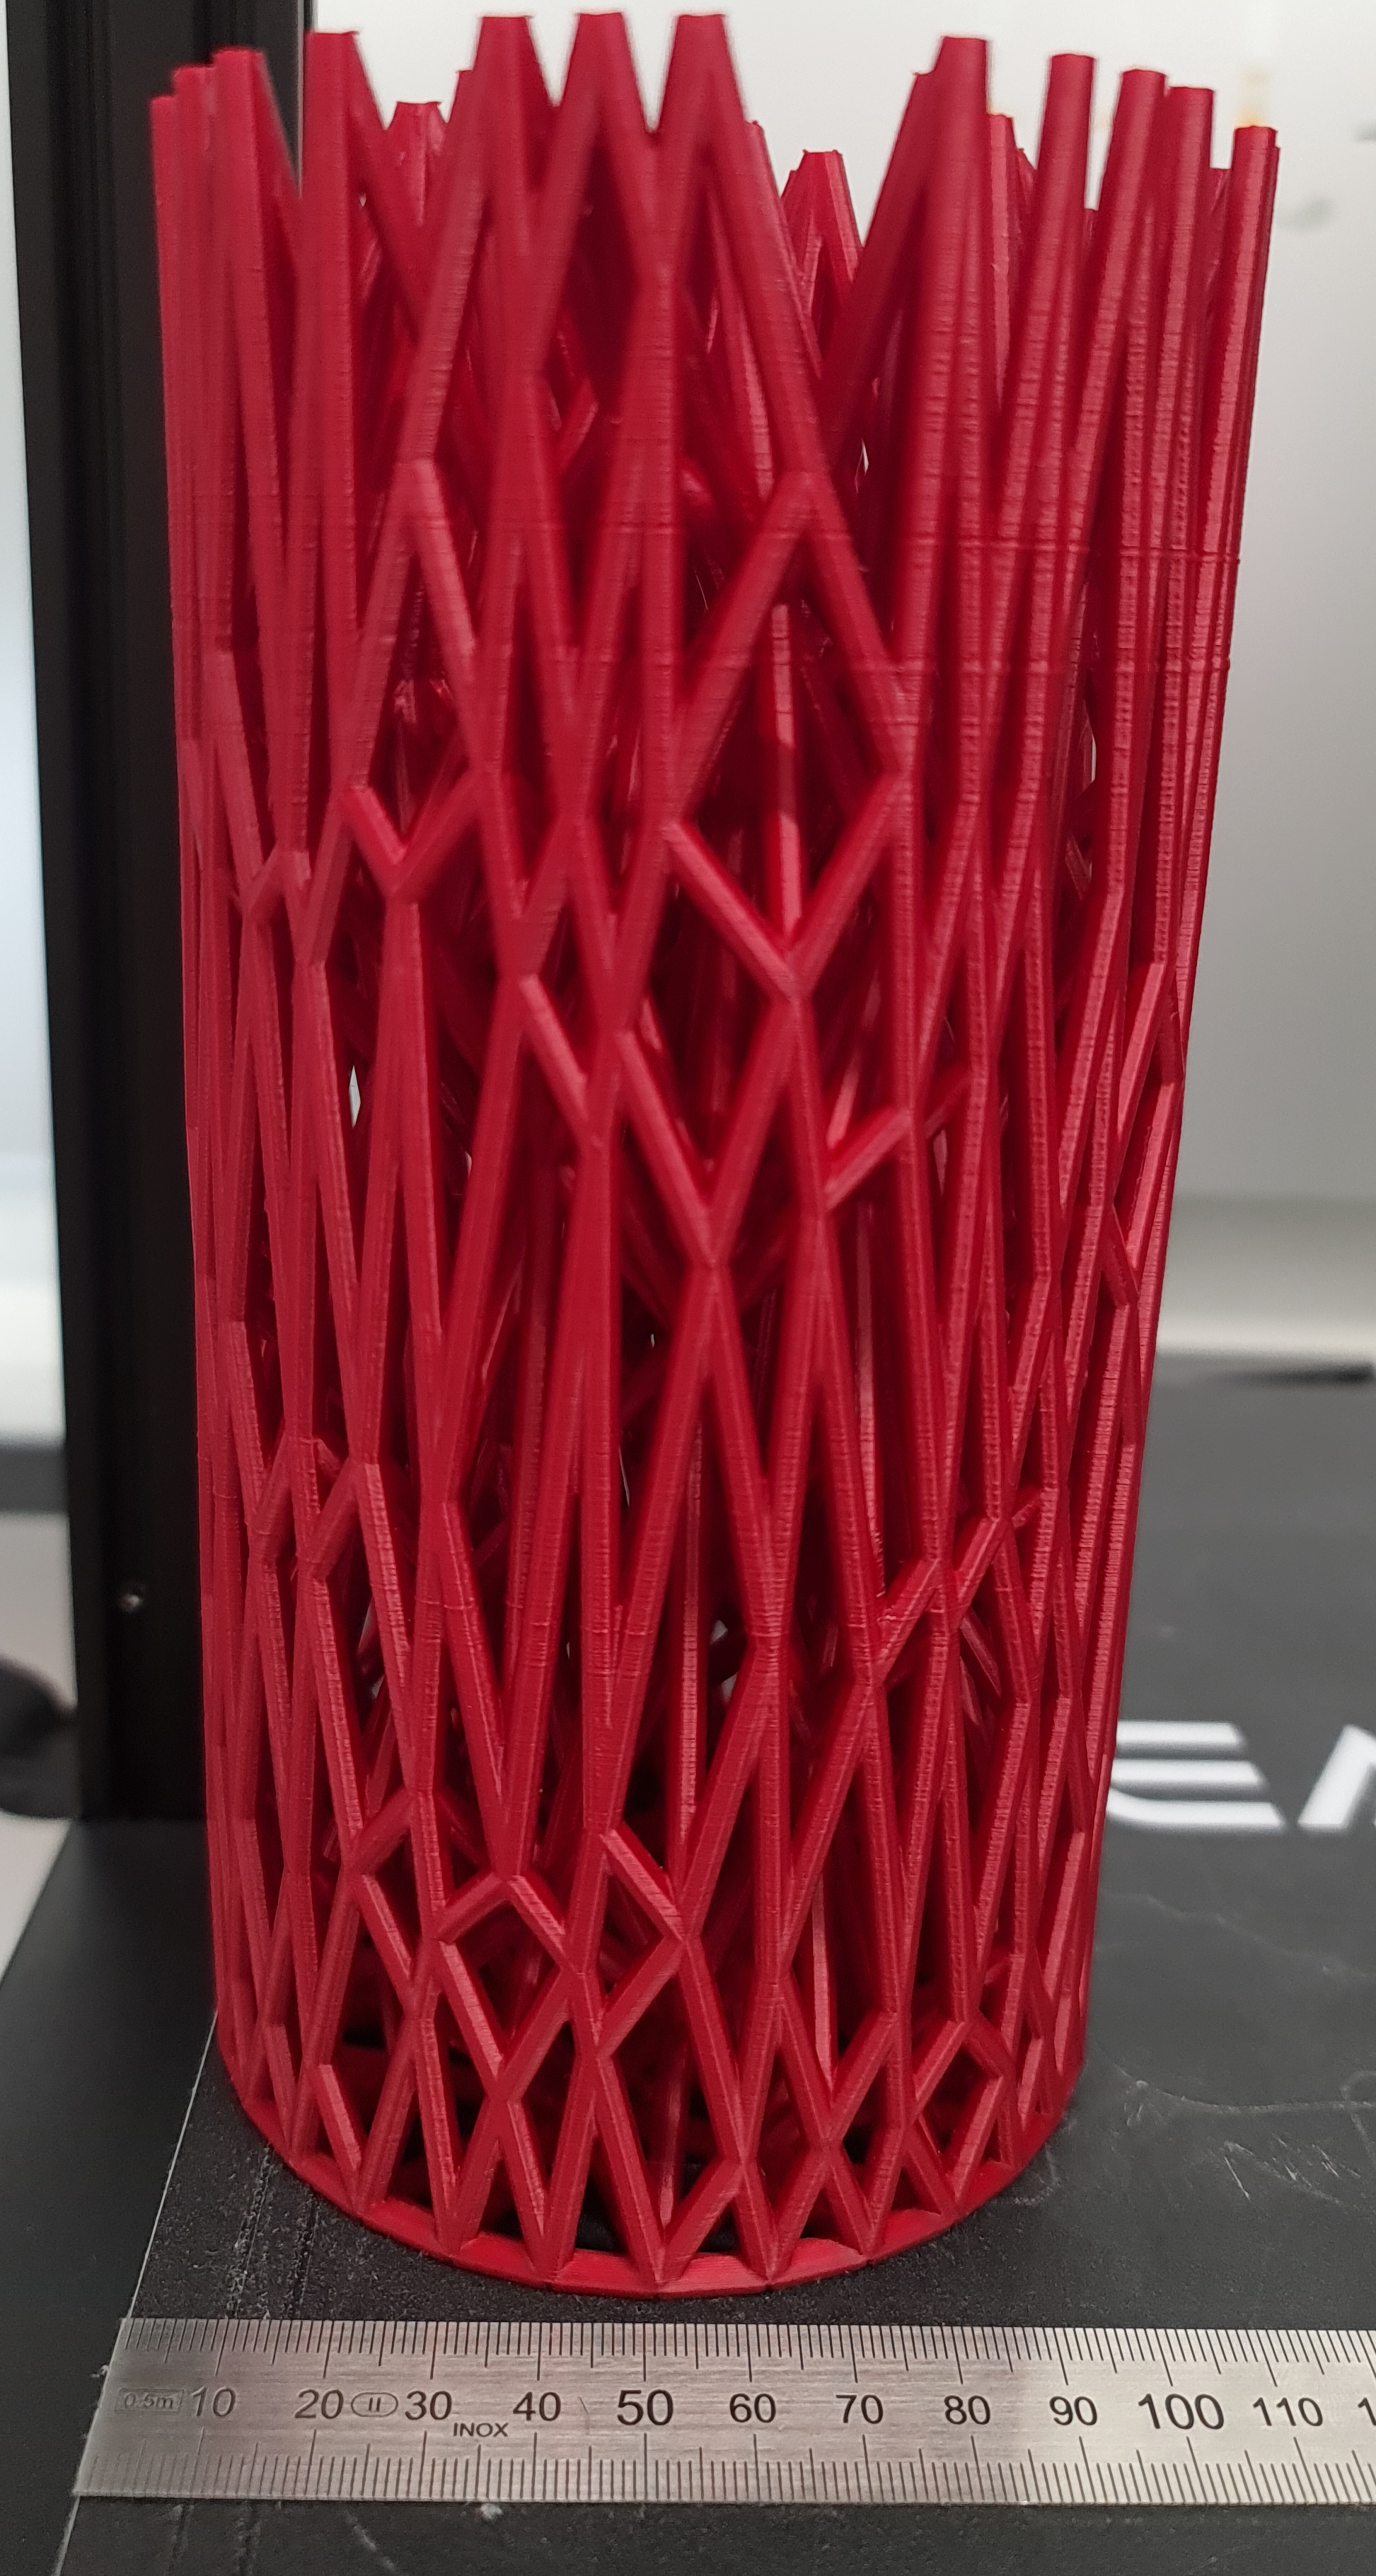
\includegraphics[width = \textwidth]{imgs/large_1.png}
     \end{subfigure}
     \hspace{0.3cm}
    \begin{subfigure}[t]{0.31\textwidth}
        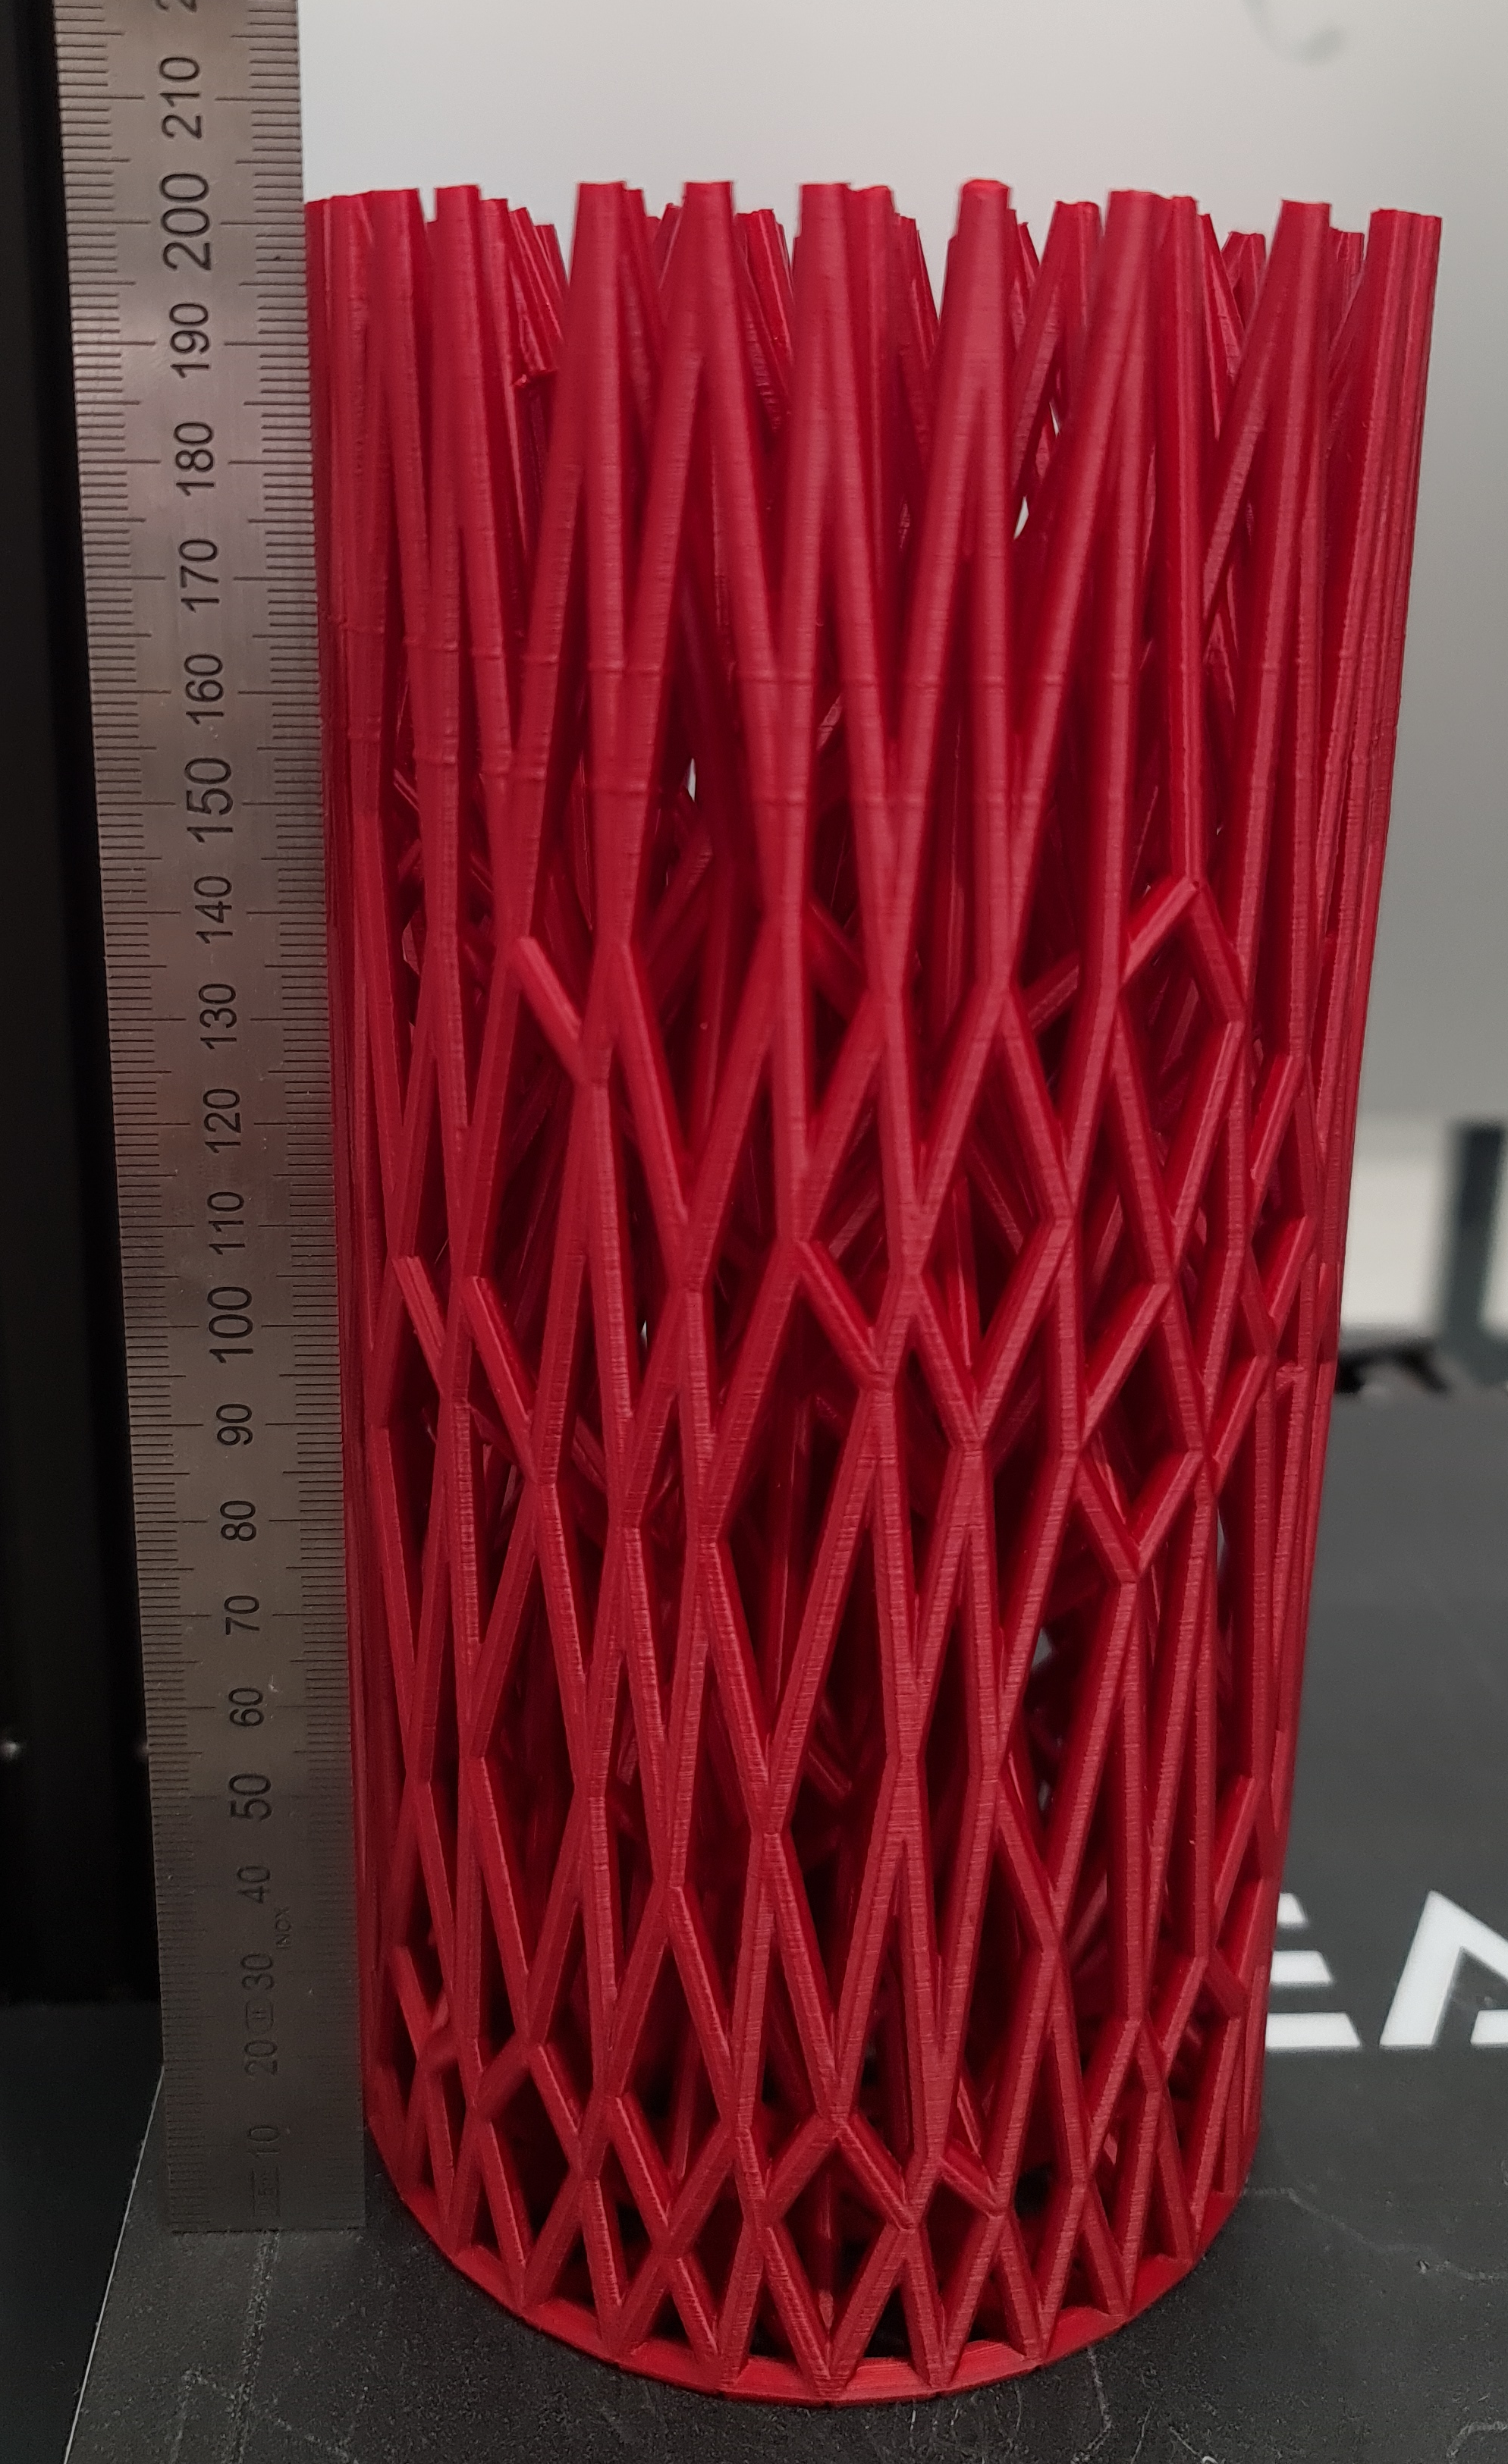
\includegraphics[width =\textwidth]{imgs/large_2.png}
     \end{subfigure}
     \caption{Example of a structure created from a cylinder 20 cm high and 10 cm in diameter}
    \label{fig:large}
\end{figure}


\begin{figure}[!htbp]
    \centering
    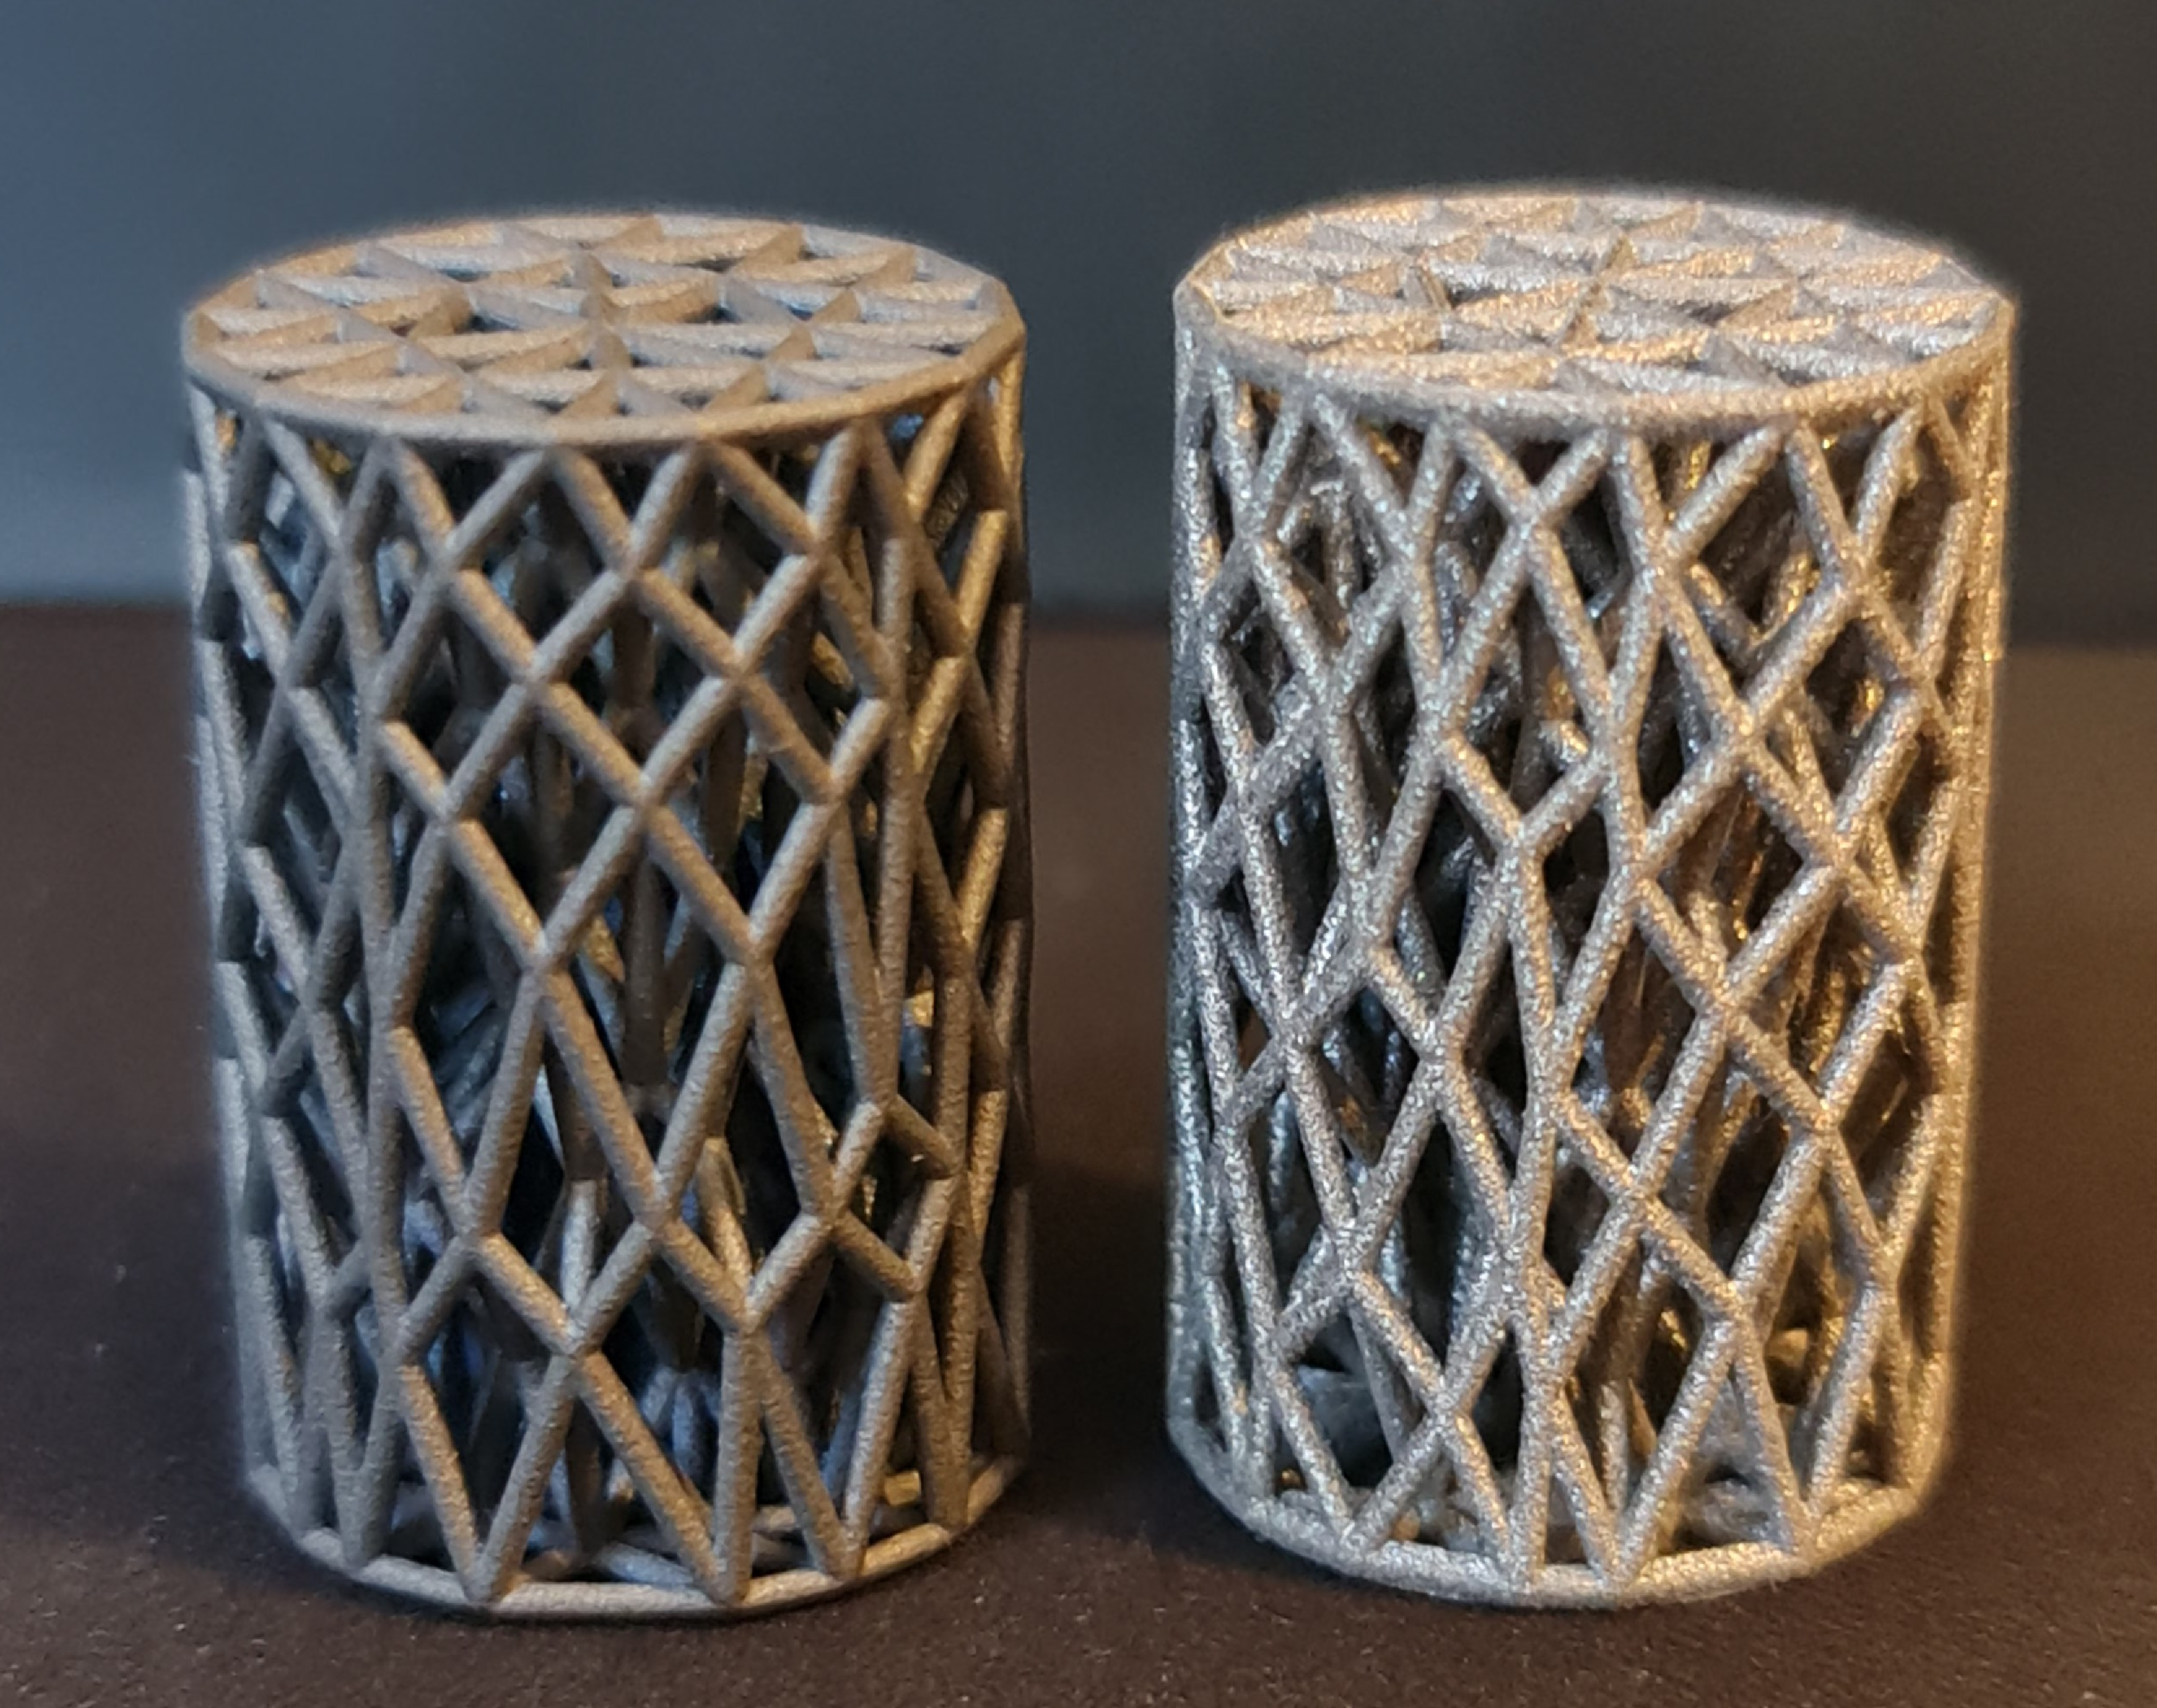
\includegraphics[width= 0.9\textwidth]{imgs/metal.png}
    \caption{Structures printed using LPBF. The sample on the left underwent the annealing process, while the one on the right did not.}
    \label{fig:metal}
\end{figure}

\end{document}